\documentclass{article}

% preambulo:
\input{Control_tp1_preamble.tex}

\begin{document}

\newgeometry{} % margenes default para la caratula
% caratula:
\begin{titlepage}
\newcommand{\HRule}{\rule{\linewidth}{0.5mm}}
\center
\mbox{\textsc{\LARGE \bfseries {Instituto Tecnol\'ogico de Buenos Aires}}}\\[1.5cm]
\textsc{\Large 22.85 - Sistemas de Control}\\[0.5cm]


\HRule \\[0.6cm]
{ \Huge \bfseries Trabajo de Laboratorio N$^{\circ}$1: Phase-Locked Loop (PLL) o Lazo de Enganche de Fase}\\[0.4cm] % Title of your document
\HRule \\[1.5cm]


{\large

\emph{Grupo 1}\\
\vspace{3px}

\begin{tabular}{lr} 	
\textsc{M\'aspero}, Martina  & 57120 \\
\textsc{Mestanza}, Joaqu\'in Mat\'ias  & 58288 \\
\textsc{Nowik}, Ariel Santiago  & 58309 \\
\textsc{Panaggio Venerandi}, Guido Martin  & xxxxx \\
\textsc{Parra}, Roc\'io  & 57669 \\
\textsc{Regueira}, Marcelo Daniel  & 58300 \\

\end{tabular}

\vspace{20px}

\emph{Profesor}\\
\vspace{3px}
\textsc{Nasini}, V\'ictor Gustavo\\ 	
\vspace{100px}

\begin{tabular}{ll}

Presentado: & xx/09/2019\\

\end{tabular}

}

\vfill

\end{titlepage}

% cambio los margenes para el resto del documento
\newgeometry{left=2.5cm, top=2.5cm, right=2cm, bottom=2cm}

% indice:
\tableofcontents
\newpage

\section*{Ejercicio 1: Prelaboratorio}
\addcontentsline{toc}{section}{Ejercicio 1: Prelaboratorio}
Se pidió analizar distintas transferencias (en la sección Prelaboratorio) del diagrama en bloques del circuito provisto por la cátedra.
\begin{figure}[H]
\centering
\includegraphics[width=1\linewidth]{images/Circuito.PNG}
\caption{Diagrama en bloques del circuito}
\label{fig:Circuito}
\end{figure}

\subsection*{a) Modulador (VCO)}

\begin{equation} \label{mod_eqn}
\frac{\theta(s)}{V_{in}(s)} = \frac{K_0}{s}
\end{equation}

\subsection*{b) Demodulador (PLL)}

\begin{equation} \label{demod_eqn}
\frac{V_f(s)}{\theta(s)} = \frac{s\cdot K_d \cdot F(s)}{s+K_0K_dF(s)}
\end{equation}

\subsection*{c) Filtros pasabajos: $F_1(s)$ y $F_2(s)$}

\begin{equation} \label{f1_eqn}
F_1(s) = \frac{1}{ 1 + \frac{s}{\omega_1}
}
\qquad \text{donde} \qquad \omega_1=\frac{1}{R_5\cdot C_6} 
\end{equation}


\begin{equation} \label{f2_eqn}
F_2(s) = \frac{1+\frac{s}{\omega_2}}{ 1 + \frac{s}{\omega_{eq}}} \qquad \text{donde} \qquad \omega_2=\frac{1}{R_6\cdot C_6} \qquad \omega_{eq} = \frac{1}{\frac{1}{\omega_1} + \frac{1}{\omega_2}} 
\end{equation}


\subsection*{d) $F_0(s)$}

\begin{equation} \label{fo_eqn}
F_0(s) = \frac{V_{out}(s)}{V_f(s)} = \frac{1}{ 1 + \frac{s}{\omega_0}} \qquad \text{donde} \qquad \omega_0=\frac{1}{R_9\cdot C_7}
\end{equation}


\section*{Ejercicio 2: factor de amortiguamiento considerando los filtros}
\addcontentsline{toc}{section}{Ejercicio 2: factor de amortiguamiento considerando los filtros}

Notar que lo que cambia entre los filtros es $R_6 = 0$ así que dejamos las expresiones generales.

\begin{equation} \label{vftheta_eqn}
\frac{V_f(s)}{\theta(s)} = \frac{ s}{K_0}
\cdot \frac{ 1 + \frac{s}{\omega_2} }
{ \left(\frac{s}{\omega_n}\right)^2 + 2\frac{\xi}{\omega_n}  + 1}
\end{equation}

\begin{equation} \label{wn_eqn}
\omega_n = \sqrt{\frac{K_d K_0}{C_6\cdot(R_5+R_6)}}
\end{equation}


\begin{equation} \label{xi_eqn}
\xi = \frac{R_6 \cdot C_6\cdot K_d\cdot K_0  + 1}
{2\cdot \sqrt{C_6 \cdot K_d \cdot K_0 \cdot(R_5 + R_6)}}
\end{equation}

\section*{Ejercicio 3: Transferencia completa}
\addcontentsline{toc}{section}{Ejercicio 3: Transferencia completa}

\begin{equation} \label{voutvin_eqn}
\frac{V_{out}(s)}{V_{in}(s)} = \frac{V_{out}(s)}{V_f(s)} \cdot \frac{V_f(s)}{\theta(s)}\cdot \frac{\theta(s)}{V_{in}(s)}
\end{equation}

\begin{equation} \label{voutvin_eqn_posta}
\frac{V_{out}(s)}{V_{in}(s)} = \frac{1}{ 1 + \frac{s}{\omega_0}} 
\cdot \frac{ 1 + \frac{s}{\omega_2} }
{ \left(\frac{s}{\omega_n}\right)^2 + 2\frac{\xi}{\omega_n}  + 1} 
\end{equation}

\newpage

\section*{Laboratorio}
Para poder simular la transferencia completa se necesitan hallar los valores $K_0$ y $K_d$.
Se procedió inyectar una entrada de tensión constante a la entrada del VCO. Con eso se obtuvo la siguiente tabla:
\begin{table}[H]
	\centering
	\caption{Tabla centrada con datos desde ``VCO.csv'}
	\label{table7}
	\begin{tabular}{c c c c c}%
		\bfseries \# & $\bm{DC_{IN}(V)}$ & $\bm{freq_{out}(KHz)}$ & $\bm{K_0(rad/seg/V)}$  \\ \hline
		\csvreader[head to column names, late after line=\\]{vco.csv}{}{\thecsvrow & \dc & \f & \k}
		%DC_IN(V),freq_out(KHz),K0 ((rad/seg)/V)
		\hline
	\end{tabular}
	%
\end{table}

Como en el trabajo práctico se nos pide entrar al VCO con una señal de 0.5 Vpp y además un offset de 5V, se le da un peso mayor a las mediciones 4, 5 y 6. Con este  criterio optamos por un valor de:
\[ K_0= 1Mrad/seg/V \]

Luego, para determinar la constante $K_d$ se consultó la datasheet del CD4046 de Texas Instruments. En la misma se halló el siguiente gráfico:
\begin{figure}[H]
\centering
\includegraphics[width=0.6\linewidth]{images/Kd.jpg}
\caption{Características del comparador de fase tipo 1 (XOR)}
\label{fig:comp1}
\end{figure}
Por simple inspección nos queda como resultado
\[ K_d= \frac{V_{DD}}{\pi} \left(\frac{V}{rad}\right) \]
Con estos valores y los establecidos por la consigna podemos calcular $\xi$ y $\omega_n$ para cada caso:
\[ \xi = 0.0886 \qquad \text{donde} \qquad \omega_n = 5.6419\cdot 10^{5} rad/seg \qquad (RC) \]
Mediante el despeje de la ecuación \ref{xi_eqn} se halló que para que $\xi \approx 0.5$ se necesita una $R_6 = 1.6K\Omega$
\[ \xi = 0.5014 \qquad \text{donde} \qquad \omega_n = 5.2384\cdot 10^{5} rad/seg \qquad (RRC) \]


\newpage
\section*{Mediciones: Filtro con F1 (caso RC)}


\begin{figure}[H]
\centering
\includegraphics[width=0.8\linewidth]{images/conF1_superpuestas.PNG}
\caption{Gráfico de las mediciones superpuestas con la curva teórica (caso RC)}
\label{fig:superpF1}
\end{figure}




\begin{figure}[H]
\centering
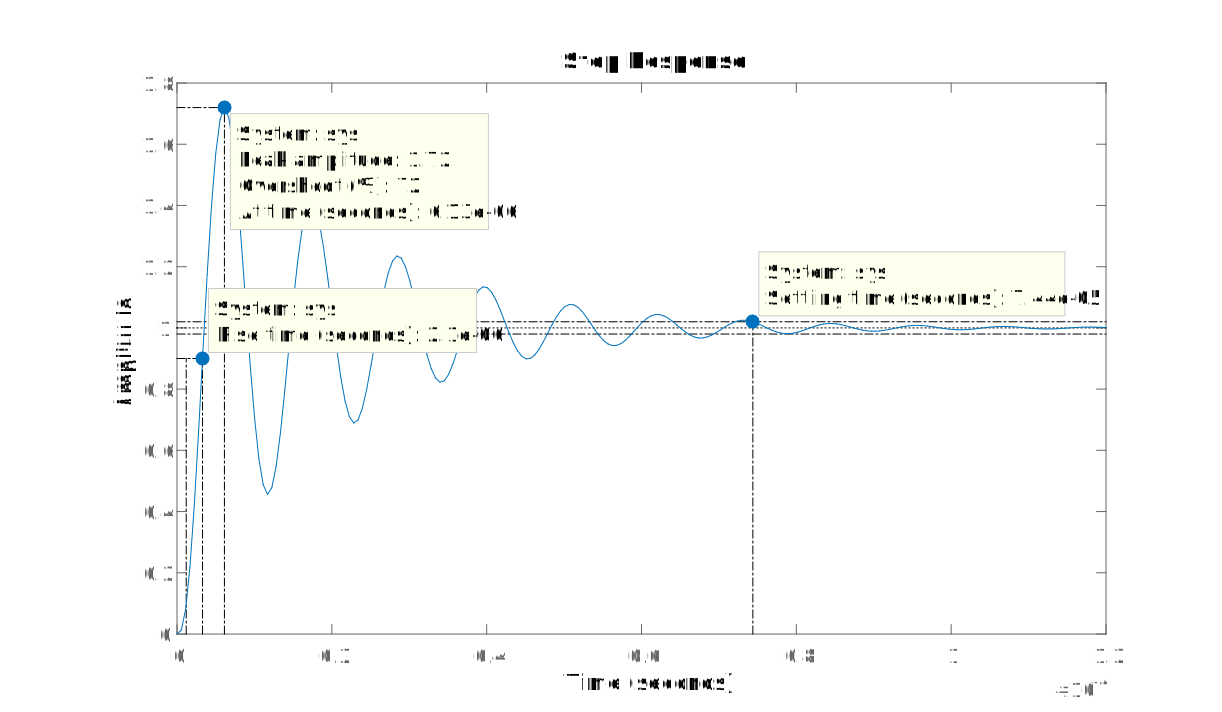
\includegraphics[width=1\linewidth]{images/todo.PNG}
\caption{Simulaciones con el primer tipo de filtro}
\label{fig:sim}
\end{figure}

\begin{figure}[H]
\centering
\includegraphics[width=0.8\linewidth]{images/os_and_trise.PNG}
\caption{Mediciones: Overshoot y rise time}
\label{fig:osandtr}
\end{figure}

\begin{figure}[H]
\centering
\includegraphics[width=0.8\linewidth]{images/tpeak_vpeak.PNG}
\caption{Mediciones: peak y peak time}
\label{fig:peak}
\end{figure}

\begin{figure}[H]
\centering
\includegraphics[width=0.8\linewidth]{images/settling_time.PNG}
\caption{Mediciones: settling time}
\label{fig:ts}
\end{figure}

\newpage

\section*{Mediciones: Filtro con F2 (caso RRC)}
\begin{figure}[H]
\centering
\includegraphics[width=0.8\linewidth]{images/conF2_superpuestas05.PNG}
\caption{Gráfico de las mediciones superpuestas con la curva teórica (caso RRC)}
\label{fig:superpF2}
\end{figure}

\begin{figure}[H]
\centering
\includegraphics[width=0.8\linewidth]{images/05vpp/simu.PNG}
\caption{simulación del circuito}
\label{fig:simu}
\end{figure}


\begin{figure}[H]
\centering
\includegraphics[width=0.8\linewidth]{images/05vpp/os_rt05vpp.PNG}
\caption{Mediciones del overshoot y risetime}
\label{fig:os_rt05vpp}
\end{figure}

\begin{figure}[H]
\centering
\includegraphics[width=0.8\linewidth]{images/05vpp/tpeak_vpeak.PNG}
\caption{medición de peak y peak time}
\label{fig:tpeak_vpeak}
\end{figure}


\begin{figure}[H]
\centering
\includegraphics[width=0.8\linewidth]{images/05vpp/settling_time.PNG}
\caption{medición de settling time}
\label{fig:settling_time}
\end{figure}


\section*{Filtro de salida}
La función que cumple el filtro de salida es fundamentalmente la de permitir obtener una señal salida mas limpia con respecto al ruido filtrando este y, ademas, eliminar las oscilaciones de alta frecuencia que pudieran no haber sido atenuadas adecuadamente por el filtro LF en cualquiera de las topologias que se presentaron para dicho filtro.
Desde un punto de vista teórico esta etapa no afectará la transferencia del PLL propiamente dicho, ya que se localiza a la salida de este, pero si tendrá influencia en la transferencia del sistema total. Según los valores propuestos para el resistor y el capacitor por la cátedra se tendrá que la constante de tiempo será de 560ns. Dicha constante afectará de forma significativa el sistema ya que cuanto menor sea esta menor será el tiempo en el que el sistema alcance el valor de la señal, pero mayor será su ancho de banda, y vice-versa.


\newpage

\section*{Conclusiones}
Se ha estudiando el proceso de diseño y las bases teóricas que sostienen el funcionamiento del PLL. Las pruebas realizadas sobre el mismo consistieron fundamentalmente en observar y analizar la respuesta dinámica del sistema al escalón realizando una comparación con los cálculos teóricos previos y las simulaciones hechas.
Al momento de operar con el filtro F1 (RC) según lo obtenido teóricamente se esperaba obtener un porcentaje de overshoot de 0.72 así como un rise time de 2.1 useg y settling time de 74.4 useg, a lo cual en la practica finalmente se obtuvo un porcentaje de 0.74, un rise time de 2.2 useg y un settling time de 81 useg. Con esto las mediciones tomadas se consideran satisfactorias. 
Por otro lado al utilizar el filtro F2 (RRC) los parámetros predichos por la teoría fueron de un overshoot de 0.24, un rise time de 2.3 useg y un settling time de 14.9 useg; pasando la practica lo que se obtuvo fue un overshoot de 0.18, un rise time de 2.5 useg y un settling time de 12.5 useg. Nuevamente se observa que los valores obtenidos representan fielmente a los obtenidos realizando el calculo teórico previo y simulado.
Con todo se pudo analizar y observar correctamente el funcionamiento del PLL como un sistema del control realimentado el cual entre otras cosas permitirá realizar la demodulacion de una señal modulada en FM, dados los parametros de trabajo adecuados, debido a dicho control que se realiza sobre la señal.

\end{document}
